\subsection{QR Code}

QR Code is an acronym for Quick Response Code, and it is a two-dimensional barcode that encodes/stores data as a block of black and white squares, developed in 1994 by Denso Wave, to track automotive parts in manufacturing. Now QR codes are one of the most used markers due to the huge support by different devices and libraries, their simplicity and ease of use, and their ability of storing large amounts of data compared to traditional barcodes.

\begin{figure}[h]
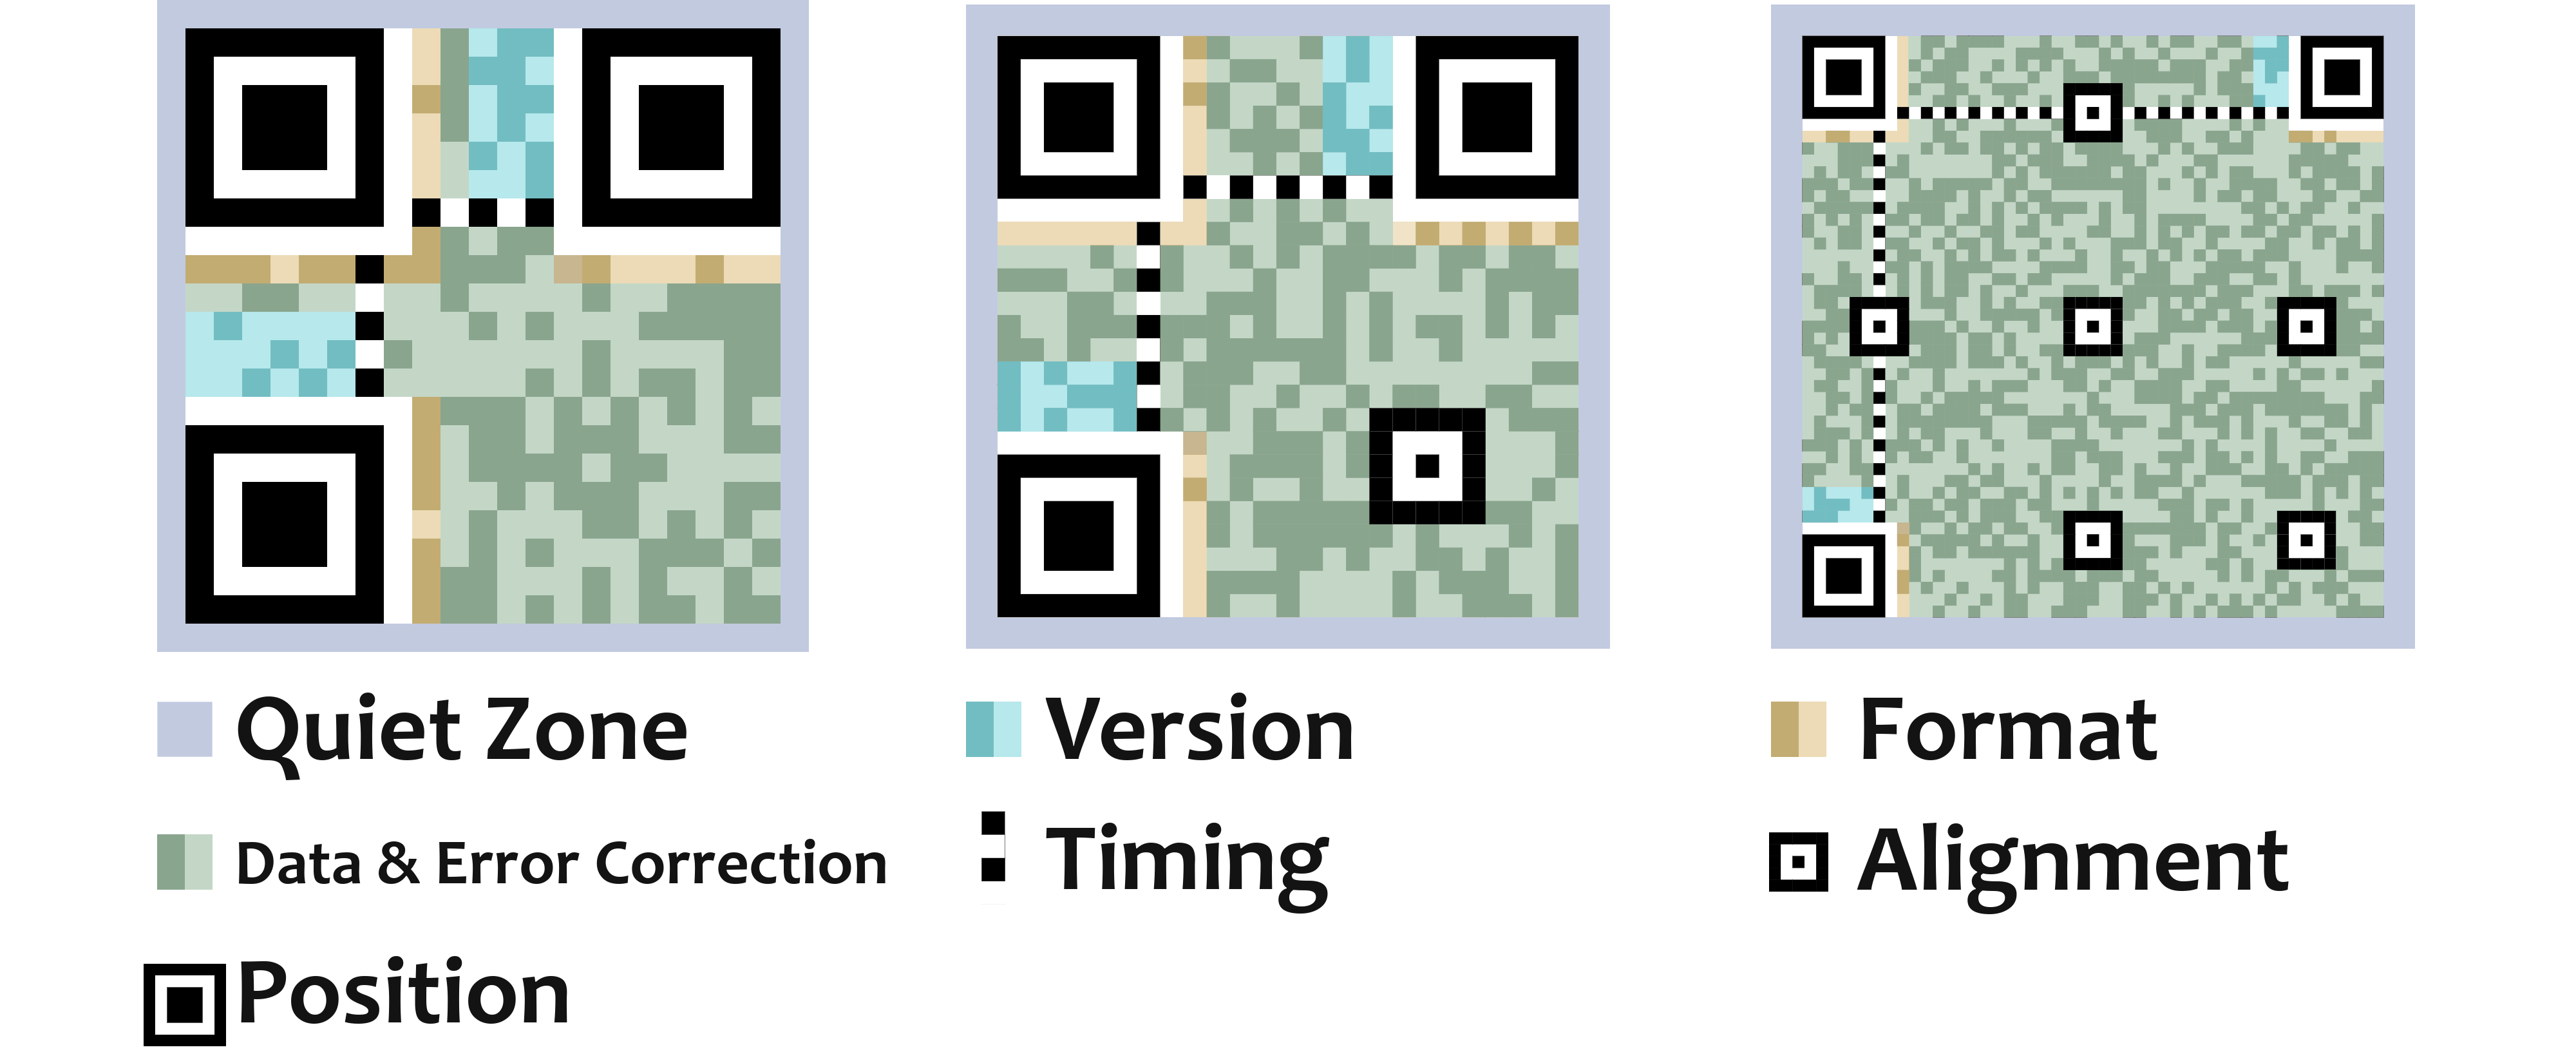
\includegraphics[width=\textwidth]{assets/ch2/QR Codes Figure.png}
\caption{These are three QR Codes that store texts. The texts' lengths get larger going from the left to the right. Notice that the alignment patter only appears at the bigger QR Codes, and there are multiple ones at the biggest QR Code. }
\end{figure}

All QR Codes have standard structure as shown in Figure 2.1. This structure is made out of the following parts:

\begin{itemize}
	\item \textbf{Quiet Zone:} This is a white empty area surrounds the QR Code that helps distinguishing it from its surroundings.
	\item \textbf{Version Information:} QR Codes have different versions/sizes which specified these two areas.
	\item \textbf{Format Information:} This part contains data about the error tolerance and mask pattern used.
	\item \textbf{Data \& Error Correction:} This is where the encoded data, and the error correction are.
	\item \textbf{Timing Patterns:} Helps identifying squares and determining the matrix's size.
	\item \textbf{Alignment Marker:} Ensures the code can be read even if it is skewed or scanned from an angle.
	\item \textbf{Positions Markers:} Help the scanner recognize the code, read it fast, and determining the code's orientation.
\end{itemize}